\documentclass[a4paper]{ltxdoc}%
\usepackage[english]{babel}%
\usepackage[latin1]{inputenc}%
\usepackage[T1]{fontenc}%
\usepackage{textcomp}%
\usepackage{lmodern}%
\usepackage{bera}%
\usepackage{microtype}%
\usepackage{attachfile}%
\usepackage{ltxdocext}%
\usepackage{marginnote}%
\usepackage{metalogo}%
\usepackage[svgnames,rgb]{xcolor}%
\usepackage{amsmath,array}%
\usepackage{tikz}%
\usetikzlibrary{calc}%
\usepackage{ragged2e}%
\usepackage{url}%
\usepackage[automark,nouppercase]{scrpage2}
\usepackage{pdfcomment}%
%
\makeatletter
\setlength{\headheight}{1.1\baselineskip}%
%
\hypersetup{colorlinks=true,urlcolor=NavyBlue,linkcolor=NavyBlue,citecolor=CornflowerBlue,naturalnames=true,hypertexnames=false}%
\renewcommand{\maketitle}%
{%
  \thispagestyle{empty}%
  \pagecolor{Ivory}%
  \begin{titlepage}%
    \begin{tikzpicture}[remember picture,overlay]%
      \node[yshift=-2cm] at (current page.north west)%
      {%
        \begin{tikzpicture}[remember picture, overlay]%
          \draw[fill=CornflowerBlue,color=CornflowerBlue] (0,0) rectangle%
            (\paperwidth,2cm);%
          \draw[anchor=west,yshift=-4cm,xshift=3cm,color=NavyBlue] (0,0) node%
            {\parbox{15cm}{\RaggedRight\Huge\sffamily\textbf{\@title}}};%
          \draw[anchor=west,yshift=-6cm,xshift=3cm,color=NavyBlue] (0,0) node%
            {\parbox{15cm}{\huge\sffamily\textbf{\@fileversion}}};%
          \draw[anchor=west,yshift=-9cm,xshift=3cm,color=NavyBlue] (0,0) node%
            {\parbox{15cm}{\RaggedRight\huge\sffamily\textbf{\@subtitle}}};%
          \draw[anchor=west,yshift=-14cm,xshift=3cm,color=NavyBlue] (0,0) node%
            {\parbox{15cm}{\huge\sffamily\textbf{\@date}}};%
          \draw[anchor=west,yshift=-20cm,xshift=3cm,color=NavyBlue] (0,0) node%
            {\parbox{15cm}{\Large\sffamily{\@authorline\\\textbf{\@author}}}};%
        \end{tikzpicture}%
      };%
      \node[yshift=0cm] at (current page.south west)%
      {%
        \begin{tikzpicture}[remember picture, overlay]%
          \draw[fill=NavyBlue,color=NavyBlue,yshift=6cm,xshift=2cm] (0,0) rectangle (0.2cm,19cm);%
          \draw[fill=CornflowerBlue,color=CornflowerBlue] (0,0) rectangle (\paperwidth,2cm);%
          \draw[anchor=west,yshift=1cm,xshift=3cm,color=NavyBlue] (0,0) node%
            {\parbox{15cm}{\large\sffamily{\@refline}}};%
        \end{tikzpicture}%
      };%
    \end{tikzpicture}%
  \end{titlepage}%
  \pagecolor{white}%
}%
%
\newcommand*{\@tikzhead}[1]%
{%
  \begin{tikzpicture}[remember picture,overlay]%
    \node[yshift=-2cm] at (current page.north west)%
    {%
      \begin{tikzpicture}[remember picture, overlay]%
        \draw[fill=CornflowerBlue] (0,0) rectangle (\paperwidth,2cm);%
        \draw[anchor=west,yshift=1cm,xshift=1.5cm,color=NavyBlue] (0,0) node%
          {\parbox{15cm}{\LARGE\sffamily\textbf{\@title}}};%
        \node[anchor=east,xshift=.9\paperwidth,rectangle,%
              rounded corners=15pt,inner sep=11pt,fill=NavyBlue]%
              {\color{white}\textsc{#1}};%
      \end{tikzpicture}%
    };%
  \end{tikzpicture}%
}%
\clearscrheadings%
\ihead{\@tikzhead{\headmark}}%
\cfoot{\upshape\thepage}%
\pagestyle{scrheadings}%
%
%\newcommand*{\headline}[1]{\@mkboth{\MakeUppercase{#1}}{\MakeUppercase{#1}}}%
\newcommand*{\Headline}[1]{\@mkboth{#1}{#1}}%
%
\renewcommand{\headfont}{\normalfont\mdseries\scshape}
%
\gdef\@subtitle{}%
\providecommand*{\Subtitle}[1]{\gdef\@subtitle{#1}}%
\gdef\@fileversion{}%
\providecommand*{\Fileversion}[1]{\gdef\@fileversion{#1}}%
\gdef\@author{}%
\providecommand*{\Author}[1]{\gdef\@author{#1}}%
\gdef\@authorline{Package author:}%
\providecommand*{\Authorline}[1]{\gdef\@authorline{#1}}%
\gdef\@refline{}%
\providecommand*{\Refline}[1]{\gdef\@refline{#1}}%
\gdef\and{\unskip{}, }%
\newcommand\doubledash{-\kern0.5pt-}
\def\enoteformat{\rightskip\z@ \leftskip\z@ \parindent=1em\leavevmode\llap{\makeenmark}}
\makeatother
%
\def\LinkExMath{\href{http://mirror.ctan.org/macros/latex/contrib/pdfcomment/doc/example_math_markup.pdf}{\texttt{example\_math\_markup.pdf}}}
\def\LinkEx{\href{http://mirror.ctan.org/macros/latex/contrib/pdfcomment/doc/example.pdf}{\texttt{example.pdf}}}
\def\filename{pdfcomment.sty}%
\def\XeLaTeX{Xe\LaTeX}%
%
\makeatletter%
\renewcommand\tableofcontents%
{%
  %\section*{\contentsname}%
  \@mkboth{%
  \MakeUppercase\contentsname}{\MakeUppercase\contentsname}%
  \@starttoc{toc}%
}%
%
\newcommand\styleoption{\name@idx{style option}}%
\newcommand\stylename{\name@idx{document style}}%
\def\name@idx#1#2{%
 {\ttfamily#2}%
 \index{#2\space#1=\string\ttt{#2}\space#1}\index{#1>#2=\string\ttt{#2}}%
}%
\newcommand*\margcs[1]{\marginnote{\raggedleft\scriptsize #1}}%
\newcommand*\package[1]{\texttt{#1}\index{#1=\string\ttt{#1}}}%
\newcommand*\mco[1]{\mbox{\LANGLE\itshape#1\RANGLE}\index{#1, class option value}\index{class option value>#1}}%
%
\renewcommand\@biblabel[1]{\makebox[1.5cm][l]{[#1]}}
\renewcommand*\l@subsection{\@dottedtocline{2}{1.2em}{2.3em}}
\renewcommand*\l@subsubsection{\@dottedtocline{3}{2.4em}{3.7em}}
\makeatother
%
\setlength\parindent{0pt}%
\hypersetup{pdfauthor={Josef Kleber},pdftitle={A user-friendly interface to PDF annotations},pdfsubject={Documentation for LaTeX style \filename}}%
%
\begin{document}
%\pdfcommentsetup{date=D:20101212153723+01'00'}
\date{2016/06/13}
\bibliographystyle{alphadin}
\title{\filename}%
\Subtitle{A user-friendly interface to PDF annotations}%
\author{Josef Kleber}
\Fileversion{v2.4}
\Refline{\href{mailto:pdfcomment@jklatex.de}{\texttt{pdfcomment@jklatex.de}}\\\href{http://pdfcomment.jklatex.de}{\texttt{http://pdfcomment.jklatex.de}}}
\maketitle
\Headline{Abstract}
\begin{abstract}
For a long time \texttt{pdflatex} has offered the command \cmd\pdfannot{} for inserting arbitrary PDF annotations. However, the command is presented in a form where additional knowledge of the definition of the PDF format is indispensable. This package is an answer to the -- occasional -- questions in newsgroups, about how one could use the comment function of \texttt{Adobe Reader}. At least for the writer of \LaTeX{} code, the package offers a convenient and user-friendly means of using \cmd\pdfannot{} to provide comments in PDF files. Since version v1.1, \texttt{\filename{}} also supports: 

\medskip
\noindent\hfill\texttt{\LaTeX{} $\rightarrow$ \texttt{dvips} $\rightarrow$ \texttt{ps2pdf}, \LaTeX{} $\rightarrow$ \texttt{dvipdfmx}\footnote{only with style option \texttt{dvipdfmx}} \XeLaTeX\ and \LuaLaTeX}.\hfill
\medskip

Unfortunately, support of PDF annotations by PDF viewers may vary. The reference viewer for the development of this package is \texttt{Adobe Reader}.

If you can't see this annotation \pdfcomment[author={Josef Kleber},subject={Test annotation},color=lime,hspace=20pt]{This is an annotation} you are definitely using the wrong PDF viewer!
\end{abstract}
\vfill
\begin{center}
\subsubsection*{Required packages for using \substyle{\filename}}
\fbox{\parbox[t]{.8\linewidth}{\small \package{hyperref} (v6.76a [2007/04/09]), \package{zref} (v1.8 [2007/04/22]), \package{xkeyval}, \package{etoolbox}, \package{luatex85}, \package{ifpdf}, \package{ifthen}, \package{calc}, \package{marginnote}, \package{datetime2}, \package{refcount}, \package{soulpos} and the packages loaded by them.}}
\end{center}
\vfill
\clearpage
\begin{multicols}{2}
[\section*{\contentsname}
\setlength{\columnseprule}{.5pt}
\setlength{\columnsep}{30pt}\small]
\tableofcontents
\end{multicols}
\clearpage
\Headline{Acknowledgment}
\section*{Acknowledgment}
I want to thank the following persons for contributions to the development of this package:

\begin{itemize}
\item \textbf{Javier Bezos} for the development of \package{soulpos}, which allows much better support of non standard text cases in \cs{pdfmarkupcomment}.

\item \textbf{Alexander Grahn} for contributing a patch for other drivers

\medskip
\noindent\hfill\texttt{\LaTeX{} $\rightarrow$ \texttt{dvips} $\rightarrow$ \texttt{ps2pdf}, \LaTeX{} $\rightarrow$ \texttt{dvipdfmx} and \XeLaTeX}.\hfill
\medskip

\item \textbf{Ulrike Fischer} for answering my stupid questions on d.c.t.t. for making the avatar and style system possible and much more.

\item \textbf{Christian Feuers�nger} for contributing new ideas in form of his package \package{pdfmarginpar.sty} and for solving the printing problem\footnote{see section \ref{sec:print}} of PDF annotations and popups.

\item \textbf{Ross Moore} for contributing ideas and code for his own feature request to support \texttt{\string\pdfmarkupcomment} in math mode.

\item \textbf{Heiko Oberdiek} also for answering my stupid questions on d.c.t.t., as well as for the development of dozens of very usefull packages, especially \file{hyperref.sty}, \file{hycolor.sty} and \file{zref.sty}, which made this package possible.

\item \textbf{Herbert Vo�} also for answering my stupid questions on d.c.t.t.
\end{itemize}

I also want to thank the following persons for bug reports, feature requests, ...: Til Birnstiel, Jannis von Buttlar, Gabriel Cardona, Thomas Feller, Florent Chervet, Jin-Hwan Cho, Marcel Dausend, Andrew Dawson, diabonas, Max Funk, Zvi Gilboa, Thomas K�nig, Marc-Andr� Michel, Guillaume Millet, Fritz Moore, Michael Niedermair, Stefan Pinnow, Ren� Schwarz
\clearpage
\section{Options}
\subsection{Global options}
\subsubsection[\texttt{final}]{\styleoption{final}}\label{sec:final}
The option \styleoption{final} will set the package to final mode. The PDF annotations will not be typeset and will not influence line breaking. Use the local option \styleoption{disable} if you want to disable single PDF annotations. (see: \ref{sec:disable})
\subsubsection[\texttt{draft}]{\styleoption{draft}}\label{sec:draft}
The option \styleoption{draft} (default) will set the package to draft mode. Therefore, the PDF annotations will be typeset.
\subsubsection[\texttt{dvipdfmx}]{\styleoption{dvipdfmx}}\label{sec:dvipdfmx}
If you want to use the driver \texttt{dvipdfmx} for creating your documents, you have to use the option \styleoption{dvipdfmx}. The other drivers are recognized automatically.
\subsubsection[\texttt{version}]{\styleoption{version}}\label{sec:version}
Version v2.0 of \texttt{pdfcomment.sty} introduced a bugfix that removes unwanted whitespace before the comment commands. This may also change the reference point for options like \styleoption{hoffset}. If you want to preserve the old behavior for older documents simply use \texttt{version=1}. Otherwise \texttt{version=2} is used by default! 
\subsection{Local options}
The following options are useable as options for the commands presented in sections \ref{sec:umgebungen} and \ref{sec:befehle}, as well as style options. As style options they have global effect, whereas they have only local effect when used in commands.

\subsubsection[\texttt{subject}]{\styleoption{subject}}\label{sec:subject}
You can use the option \styleoption{subject} for defining the subject of the PDF popup annotations.

\subsubsection[\texttt{author}]{\styleoption{author}}\label{sec:author}
You can use the option \styleoption{author} for defining the author of the PDF popup annotations.

\subsubsection[\texttt{opacity}]{\styleoption{opacity} (\underline{\texttt{1.0}})}\label{sec:opacity}
You can use the option \styleoption{opacity} for defining the opacity of PDF annotations with values between 0 (transparent) and 1 (not transparent). If you want to print PDF popup annotations with transparency you will have to use the option \styleoption{open}\texttt{=true}.

\subsubsection[\texttt{icon}]{\styleoption{icon} (\underline{\texttt{Comment}})}\label{sec:icon}
You can use the option \styleoption{icon} for defining the graphic used for the PDF text annotations. The following icons are defined as mandatory by the PDF reference:

\pdfcommentsetup{author={Josef Kleber},subject={Icon �bersicht},width=17mm}
{\renewcommand{\arraystretch}{2.5}
\begin{center}
\begin{tabular}{rlrlrl}
\texttt{Comment} & \pdfcomment[icon=Comment,color=Ivory,hspace=1.5cm]{options: icon=Comment,color=Ivory} &
\texttt{Key} & \pdfcomment[icon=Key,color=Khaki,hspace=1.5cm]{options: icon=Key,color=Khaki} &
\texttt{Note} & \pdfcomment[icon=Note,color=LavenderBlush,hspace=1.5cm]{options: icon=Note,color=LavenderBlush}\\
\texttt{Help} & \pdfcomment[icon=Help,color=CornflowerBlue,hspace=1.5cm]{options: icon=Help,color=CornflowerBlue} &
\texttt{NewParagraph} & \pdfcomment[icon=NewParagraph,color=SkyBlue,hspace=1.5cm]{options: icon=NewParagraph,color=SkyBlue}\\
\texttt{Paragraph} & \pdfcomment[icon=Paragraph,color=SpringGreen,hspace=1.5cm]{options: icon=Paragraph,color=SpringGreen} &
\texttt{Insert} & \pdfcomment[icon=Insert,color=PaleTurquoise,hspace=1.5cm]{options: Insert,color=PaleTurquoise} &
 & \\
\end{tabular}
\end{center}
}

\begin{samepage}
Furthermore the following icons are also supported by \texttt{Adobe Reader} and some other PDF viewers:

{\renewcommand{\arraystretch}{2.5}
\begin{center}
\begin{tabular}{rlrlrl}
\texttt{Check} & \pdfcomment[icon=Check,color=Orchid,hspace=1cm]{options: icon=Check,color=Orchid} &
\texttt{Circle} & \pdfcomment[icon=Circle,color=LightCyan,hspace=1cm]{options: icon=Circle,color=LightCyan} &
\texttt{Cross} & \pdfcomment[icon=Cross,color=Bisque,hspace=1cm]{options: icon=Cross,color=Bisque}\\
\texttt{Star} & \pdfcomment[icon=Star,color=Aquamarine,hspace=1cm]{options: icon=Star,color=Aquamarine} &
\texttt{RightArrow} & \pdfcomment[icon=RightArrow,color=Gainsboro,hspace=1cm]{options: icon=RightArrow,color=Gainsboro} &
\texttt{RightPointer} & \pdfcomment[icon=RightPointer,color=Salmon,hspace=1cm]{options: icon=RightPointer,color=Salmon}\\
\texttt{UpArrow} & \pdfcomment[icon=UpArrow,color=Teal,hspace=1cm]{options: icon=UpArrow,color=Teal} &
\texttt{UpLeftArrow} & \pdfcomment[icon=UpLeftArrow,color=Magenta,hspace=1cm]{options: icon=UpLeftArrow,color=Magenta} &
\texttt{CrossHairs (AR X)} & \pdfcomment[icon=CrossHairs,color=green,hspace=1cm]{options: icon=CrossHairs,color=green}
\end{tabular}
\end{center}
}
\end{samepage}

\subsubsection[\texttt{deadline}]{\styleoption{deadline}}\label{sec:deadline}
You can use the option \styleoption{deadline} for defining a time limit until a problem has to be solved. The deadline will be added at the end of the comment, as well as in the list of comments, if an appropriate list style is chosen.

\subsubsection[\texttt{color}]{\styleoption{color}  (\underline{\texttt{\lbrack 0 0 1\rbrack}} (blue))}\label{sec:color}
You can use the option \styleoption{color} for defining the color of PDF annotations in the form \{0.34 0.56 0.12\} (RGB). If you are using the additional package \package{xcolor} you can use predefined color names, as well as the available optional color names. Furthermore you can use the command \cmd\definecolor{} to define your own named colors. Please take a look at the attached example \file{example.tex}.\marginnote{\attachfile[author={Josef Kleber},subject={example.tex},description={source code: example.tex} ,mimetype={text/plain}, icon={Tag}]{example.tex}} It shows the different possibilities of defining colors.

By definition the PDF specification allows four different color spaces with different numbers of color values:

\begin{center}
\begin{tabular}{cl}
\# & color space\\
\hline
0 & transparent \\
1 & grey scale \\
3 & RGB\\
4 & CMYK\\
\end{tabular}
\end{center}

\subsubsection[\texttt{icolor}]{\styleoption{icolor}}\label{sec:icolor}
You can use the option \styleoption{icolor} for defining the so called 'inner color', which is used by some PDF annotations, like arrowheads or the inner area of PDF circle annotation. For the rest, the provisions of the option \styleoption{color} shall apply.

\subsubsection[\texttt{open}]{\styleoption{open}  (\texttt{true},\underline{\texttt{false}})}\label{sec:open}
You can use the option \styleoption{open} for defining the opening status of the PDF popup annotations.

If you want to print the PDF popup annotations (with transparency) you will have to use the option \styleoption{open}\texttt{=true}.

\subsubsection[\texttt{hspace}]{\styleoption{hspace}  (\underline{\texttt{0pt}})}\label{sec:hspace}
You can use the option \styleoption{hspace} for defining the horizontal space after the PDF text annotations, otherwise the PDF text annoations will overlay the text.

\subsubsection[\texttt{type}]{\styleoption{type}}\label{sec:type}
You can use the option \styleoption{type} for defining the type of PDF annotation, if a comment command supports more than one PDF annotations:

{\renewcommand{\arraystretch}{1.2}
\begin{center}
\begin{tabular}{ll}
\multicolumn{1}{c}{comment command} & \multicolumn{1}{c}{possible types}\\
\hline
\cs{pdffreetextcomment} & \underline{freetext}, callout, typewriter \\
\cs{pdflinecomment} & \underline{line}, polyline, polygon \\
\end{tabular}
\end{center}}


\subsubsection[\texttt{font}]{\styleoption{font} (\underline{\texttt{Helv}})}\label{sec:font}
You can use the option \styleoption{font} for defining the font of PDF freetext annotations, like all fonts installed in the system, which don't contain a space in their name. Although \texttt{Adobe Reader} shows these fonts as embedded, they are not embedded in reality, but the PDF file just contains a reference\footnote{Adobe Acrobat offers the possibility to embed the fonts in the PS $\rightarrow$ PDF conversion} to the font (default: Helvetica)! Therefore you should use this option quite carefully. In the case of document exchange between several authors you should just use fonts, which are available on all computer systems, like the so called  'standard 14 fonts'. \pdfcomment[icon=Help,color=blue,open=true,subject={standard 14 fonts}]{Times-Roman (TiRo), Times-Bold (TiBo), Times-Italic (TiIt), Times-BoldItalic (TiBI), Helvetica (Helv), Helvetica-Bold (HeBo), Helvetica-Oblique (HeOb), Helvetica-BoldOblique (HeBO), Courier (Cour), Courier-Bold (CoBo), Courier-Oblique (CoOb), Courier-BoldOblique (CoBO), ZapfDingbats (ZaDb), Symbol (Symb)}

\subsubsection[\texttt{fontsize}]{\styleoption{fontsize} (\underline{\texttt{12bp}})}\label{sec:fontsize}
You can use the option \styleoption{fontsize} for defining the fontsize of PDF freetext annotations.

\subsubsection[\texttt{fontcolor}]{\styleoption{fontcolor} (\underline{\texttt{\lbrack 0 0 0\rbrack}} (black))}\label{sec:fontcolor}
You can use the option \styleoption{fontcolor} for defining the font color in PDF freetext annotations, which must be a RGB color. 

\subsubsection[\texttt{line}]{\styleoption{line}}\label{sec:line}
You can use the option \styleoption{line} for defining the coordinates of lines in certain PDF annotations, e.\,g. in the form \{$x_1$\space$y_1$\space$x_2$\space$y_2$\}. The origin is in the bottom left page corner. The given numbers will be interpreted as Postscript points (\LaTeX{} unit: bp (big points)), as usual in PDF documents.

{\renewcommand{\arraystretch}{1.2}
\begin{center}
\begin{tabular}{ll}
\multicolumn{1}{c}{type of line} & \multicolumn{1}{c}{\# points}\\
\hline
line & $n = 2$ \\
polyline, polygon & $n > 2$ \\
callout line & $n = 3$ \\
\end{tabular}
\end{center}}

In general, the points must be given from line begin to line end. For callout lines the points must be given from line end to line begin. Please note the example file \LinkEx!

To avoid the method 'trail and error' you can load the PDF file with the Ghostscript viewer, which is capable of showing the cursor position in its status line.

\subsubsection[\texttt{linewidth}]{\styleoption{linewidth} (\underline{\texttt{1bp}})}\label{sec:linewidth}
You can use the option \styleoption{linewidth} for defining the line width of PDF annoations.

\subsubsection[\texttt{linebegin}]{\styleoption{linebegin} (\underline{\texttt{/None})}}\label{sec:linebegin}
You can use the option \styleoption{linebegin} for defining the arrow type at the line begin. The example file \LinkEx{} shows all possible types of arrows. \pdfcomment[icon=Help,color=blue,open=true,subject={arrow types}]{/None, /Square, /Circle, /Diamond, /OpenArrow, /ClosedArrow, /Butt (PDF1.5), /ROpenArrow (PDF1.5), /RClosedArrow (PDF1.5), /Slash (PDF1.6)} 


\subsubsection[\texttt{lineend}]{\styleoption{lineend} (\underline{\texttt{/OpenArrow}})}\label{sec:lineend}
You can use the option \styleoption{lineend} for defining the arrow type at the line end.

\subsubsection[\texttt{linesep}]{\styleoption{linesep} (\underline{\texttt{0.5cm}})}\label{sec:linesep}
You can use the option \styleoption{linesep} for defining the horizontal space between text and line in the command \cs{pdfsidelinecomment}.

\subsubsection[\texttt{borderstyle}]{\styleoption{borderstyle} (\underline{\texttt{solid}},\texttt{dashed})}\label{sec:borderstyle}
You can use the option \styleoption{borderstyle} for defining the line style.

\subsubsection[\texttt{dashstyle}]{\styleoption{dashstyle} (\underline{\texttt{\{3 3\}}})}\label{sec:dashstyle}
You can use the option \styleoption{dashstyle} for defining the dash style, e.\,g. \{5 3\} (5 points line, 3 points space).

\subsubsection[\texttt{bse}]{\styleoption{bse} (\underline{\texttt{none}},\texttt{cloudy})}\label{sec:bse}
You can use the option \styleoption{bse} for defining the 'border style effect'.

\subsubsection[\texttt{bsei}]{\styleoption{bsei} (\underline{\texttt{1}})}\label{sec:bsei}
You can use the option \styleoption{bsei} for defining the 'border style effect intensity' (size of cloud elements). The PDF reference suggests values between 1 and 2. 

\subsubsection[\texttt{caption}]{\styleoption{caption} (\texttt{none},\underline{\texttt{inline}},\texttt{top})}\label{sec:caption}
You can use the option \styleoption{caption} for defining the caption type of lines.

The options \styleoption{inline} and \styleoption{top} shows the comment 'inline' and on top of the line. While using \styleoption{none} the comment will be shown in a PDF popup annotation. 

\subsubsection[\texttt{captionhoffset}]{\styleoption{captionhoffset} (\underline{\texttt{0pt}})}\label{sec:captionhoffset}
You can use the option \styleoption{captionhoffset} for defining a horizontal offset, that is a horizontal shift of the line caption.

\subsubsection[\texttt{captionvoffset}]{\styleoption{captionvoffset} (\underline{\texttt{0pt}})}\label{sec:captionvoffset}
You can use the option \styleoption{captionvoffset} for definig a vertical offset of the line caption.

\subsubsection[\texttt{voffset}]{\styleoption{voffset} (\underline{\texttt{0pt}})}\label{sec:voffset}
You can use the option \styleoption{voffset} for defining a vertical offset of the PDF annotations, that is a vertical shift for the given length.

\subsubsection[\texttt{hoffset}]{\styleoption{hoffset} (\underline{\texttt{0pt}})}\label{sec:hoffset}
You can use the option \styleoption{hoffset} for defining a horizontal offset of the PDF annotations.

\subsubsection[\texttt{width}]{\styleoption{width} (\underline{\texttt{0pt}})}\label{sec:width}
You can use the option \styleoption{width} for defining the width of PDF annotations, e.\,g. the width of FreeText annotations. PDF text annatations have a width of 0pt by definition.

\subsubsection[\texttt{height}]{\styleoption{height} (\underline{\texttt{0pt}})}\label{sec:height}
You can use the option \styleoption{height} for definig the height of PDF annotations. PDF text annatations have a height of \cmd\normalbaselineskip{} by definition.

\subsubsection[\texttt{markup}]{\styleoption{markup} (\underline{\texttt{Highlight}},\texttt{Underline},\texttt{Squiggly},\texttt{StrikeOut})}\label{sec:markup}
You can use the option \styleoption{markup} for defining the type of the PDF text markup annotation.

\subsubsection[\texttt{disable}]{\styleoption{disable} (\texttt{true},\underline{\texttt{false})}}\label{sec:disable}
You can use the option \styleoption{disable} for switching off single PDF annotation. For switching off all PDF annotations use the global option \styleoption{final}.

\subsubsection[\texttt{date}]{\styleoption{date}}\label{sec:date}
You can use the option \styleoption{date} to assign a date to PDF annotations. If no explicit date is assigned the date and time of the creation of the PDF document is used. The input has to be in PDF date format, e.g.:

\begin{center}
\begin{tabular}{l}
\texttt{D:YYYYMMDDhhmmss+TZ}\\
\texttt{D:20101224153657+01'00'}
\end{tabular}
\end{center}

\subsubsection[\texttt{timezone}]{\styleoption{timezone} (\underline{\texttt{+00'00'}})}\label{sec:timezone}
You only have to use the option \styleoption{timezone}, if you are using automatic date setting and \XeLaTeX. Otherwise the \texttt{pdflatex} primitive \string\pdfcreationdate\ will be used. \styleoption{timezone}=+01'00' sets the timezone to central european time CET (default: +00'00' (GMT)).

\subsubsection[\texttt{avatar}]{\styleoption{avatar}}\label{sec:avatar}
With the option \styleoption{avatar} you can load the option lists, that were predefined with the command \cmd\defineavatar{} to avoid annoying typing. 

\subsubsection[\texttt{style}]{\styleoption{style}}\label{sec:style}
With the option \styleoption{style} you can also load predefined option lists for spliting personal and stylistic options, e.\,g. \texttt{avatar=Josef, style=MyComment}.

\subsubsection[\texttt{mathstyle}]{\styleoption{mathstyle} (\underline{\texttt{\string\textstyle}})}\label{sec:mathstyle}
With the option \styleoption{mathstyle} you can correct the wrong size of PDF annotations produced with \texttt{\string\pdfmarkupcomment} or \texttt{\string\pdftooltip} in math mode by setting the math style to \texttt{\string\textstyle}, \texttt{\string\displaystyle}, \texttt{\string\scriptstyle} or \texttt{\string\scriptscriptstyle}. This option is only defined for \texttt{\string\pdfmarkupcomment} and \texttt{\string\pdftooltip}, so you can not set it globally! 

\subsubsection[\texttt{printSOfinal}]{\styleoption{printSOfinal} (\underline{\texttt{true}},\texttt{false})}\label{sec:printSOfinal}
With the option \styleoption{printSOfinal} you can automatically delete PDF StrikeOut markup annotations including the text while using one of the options \styleoption{final} or \styleoption{disable}.

\section{Environments}\label{sec:umgebungen}

\subsection{Comment environments}\label{sec:kommentarumgebungen}

\subsubsection{\texorpdfstring{\cs{pdfsidelinecomment}}{\textbackslash pdfsidelinecomment}}
\label{sec:sidelinecomment}
Possible \marginnote{\raggedleft\scriptsize\envb{pdfsidelinecomment}\\\oarg{options}\marg{comment}\\\dots\\\enve{pdfsidelinecomment}}options: \styleoption{avatar}, \styleoption{style}, \styleoption{subject}, \styleoption{author}, \styleoption{color}, \styleoption{icolor}, \styleoption{opacity}, \styleoption{linewidth}, \styleoption{linebegin}, \styleoption{lineend}, \styleoption{linesep}, \styleoption{borderstyle}, \styleoption{dashstyle}, \styleoption{caption}, \styleoption{captionhoffset}, \styleoption{captionvoffset}, \styleoption{disable}, \styleoption{date}, \styleoption{timezone}

\bigskip
With the environment \env{pdfsidelinecomment} you can comment complete parts of a page in the form of two lines in the margins.

\hspace*{0pt}\newline
\begin{pdfsidelinecomment}[color=red,icolor=yellow,linebegin=/Circle,lineend=/Circle,linewidth=3bp,linesep=1cm]{ Please note }
Limitations:

\begin{itemize}
\item The PDF sideline annotation must not be longer than one page, otherwise the recognition of the page break will fail.
\item While using dvi files in the meantime you have to use a \LaTeX{} distribution, which is using \texttt{pdf(e)latex} as engine in a version $\geq$ v1.40.0\footnote{older versions are not capable of providing x/y coordinates of the current position in dvi mode.}!
\item While using \XeLaTeX{} you have to make sure that page dimensions are written to the xdvi file, e.\,g. with the option \styleoption{pagesize} of the KoMa-Script classes, or as option of the package \package{typearea.sty} respectively.
\end{itemize}
\end{pdfsidelinecomment}

\section{Commands}\label{sec:befehle}

\subsection{Comment commands}\label{sec:kommentarbefehle}

You can use the following commands for commenting your documents.

\subsubsection{\texorpdfstring{\cs{pdfcomment}}{\textbackslash pdfcomment}}
\label{sec:pdfcomment}
Possible \margcs{\cmd\pdfcomment\\\oarg{options}\marg{comment}}options: \styleoption{avatar}, \styleoption{style}, \styleoption{subject}, \styleoption{author}, \styleoption{icon}, \styleoption{color}, \styleoption{opacity}, \styleoption{open}, \styleoption{hspace}, \styleoption{voffset}, \styleoption{hoffset}, \styleoption{disable}, \styleoption{date}, \styleoption{timezone}

\bigskip
\cmd\pdfcomment{} will typeset an annotation into the text at the current \pdfcommentsetup{subject={\textbackslash pdfcomment test},hspace=18pt}\pdfcomment[icon=Star,color=YellowGreen]{This is a comment in the text} position.

Internally, the argument \marg{comment} needs to be converted to PDFDocEncoding/PDFUnicode\footnote{\cmd\hypersetup\{unicode\}}. Some chars with special meaning in \LaTeX{} (\texttt{\&}, \texttt{\%,} ...) must be escaped or replaced with their command form, e.\,g. \texttt{\string\_} or \texttt{\string\textunderscore}. Furthermore there are some commands for formatting:

\begin{center}
\begin{tabular}{cl}
\hline
\cmd\textHT & horizontal tab \\
\cmd\textLF & line feed \\
\cmd\textCR & carriage return \\
\hline
\end{tabular}
\end{center}

\subsubsection{\texorpdfstring{\cs{pdfmargincomment}}{\textbackslash pdfmargincomment}}
\label{sec:pdfmargincomment}
Possible \margcs{\cmd\pdfmargincomment\\\oarg{options}\marg{comment}}options: \styleoption{avatar}, \styleoption{style}, \styleoption{subject}, \styleoption{author}, \styleoption{icon}, \styleoption{color}, \styleoption{opacity}, \styleoption{open}, \styleoption{hspace}, \styleoption{voffset}, \styleoption{hoffset}, \styleoption{disable}, \styleoption{date}, \styleoption{timezone}

\bigskip
\cmd\pdfmargincomment{} will typeset an annotation into the margin. Please note the positioning of the annotation in this example. This documentation was written with the \LaTeX{} class \texttt{ltxdoc}\pdfcommentsetup{subject={\textbackslash pdfmargincomment test}}\pdfmargincomment[icon=Help,color=DeepPink,hspace=-30pt]{This is a comment in the margin}. Therefore the annotation is typeset into the left margin.

\subsubsection{\texorpdfstring{\cs{pdfmarkupcomment}}{\textbackslash pdfmarkupcomment}}
\label{sec:pdfmarkupcomment}
Possible \margcs{\cmd\pdfmarkupcomment\oarg{options}\\\marg{markup text}\marg{comment}}options: \styleoption{avatar}, \styleoption{style}, \styleoption{subject}, \styleoption{author}, \styleoption{color}, \styleoption{opacity}, \styleoption{markup}, \styleoption{mathstyle}, \styleoption{disable}, \styleoption{date}, \styleoption{timezone}

\bigskip
\cmd\pdfmarkupcomment{} will typeset so called PDF text markup annotations over the text specified in the argument \marg{markup text}. Possible types for the option \styleoption{markup} are: \pdfcommentsetup{subject={\textbackslash pdfmarkupcomment test}}\pdfmarkupcomment[color=yellow,markup=Highlight]{Highlight}{This is a Highlight markup annotation!}, \pdfmarkupcomment[color=red,markup=Underline]{Underline}{This is a Underline markup annotation!}, \pdfmarkupcomment[color=Teal,markup=Squiggly]{Squiggly}{This is a Squiggly markup annotation!} and \pdfmarkupcomment[color=red,markup=StrikeOut]{StrikeOut}{This is a StrikeOut markup annotation!}

\hspace*{0pt}\newline
Limitations:

\begin{itemize}
\item As the name PDF text markup annotation might lead to suggest, this form of comment is suitable for text only.
\item The specified text with the argument \marg{markup text} must not be longer than one paragraph.
\item The PDF text markup annotation must not be longer than one page, otherwise the recognition of the page break will fail.
\item While using dvi files in the meantime you have to use a \LaTeX{} distribution, which is using \texttt{pdf(e)latex} as engine in a version $\geq$ v1.40.0\footnote{older versions are not capable of providing x/y coordinates of the current position in dvi mode.}!
\item While using \XeLaTeX{} you have to make sure that page dimensions are written to the xdvi file, e.\,g. with the option \styleoption{pagesize} of the KoMa-Script classes, or as option of the package \package{typearea.sty} respectively.
\end{itemize}

Since version v1.6, \texttt{\string\pdfmarkupcomment} is also supported in math mode. So you can also comment formula like:

\definestyle{mathpopup}{author={},subject={},color=NavajoWhite,markup=Highlight}

\[
\begin{array}{c>{\displaystyle}c}
 \text{ Bernoulli Trials: } &
 \pdfmarkupcomment[style=mathpopup]{P(E)}{Probability of event E: Get exactly k heads in n coin flips.}%
  =
 \pdfmarkupcomment[style=mathpopup]{\dbinom{n}{k}}{Number of ways to get exactly k heads in n coin flips}%
  {\pdfmarkupcomment[style=mathpopup]{p}{Probability of getting heads in one flip}%
}^{%
    \pdfmarkupcomment[style=mathpopup,mathstyle=\scriptstyle]{k}{Number of heads}
  }%
 \pdfmarkupcomment[style=mathpopup]{(1-p)}{Probability of getting tails in one flip}^{%
 \pdfmarkupcomment[style=mathpopup,mathstyle=\scriptstyle]{n-k}{Number of tails}%
 }%
\end{array}
\]

Also see \LinkExMath{} for a more detailed explanation of the possibilities!
 
\subsubsection{\texorpdfstring{\cs{pdffreetextcomment}}{\textbackslash pdffreetextcomment}}
\label{sec:pdffreetextcomment}
Possible \margcs{\cmd\pdffreetextcomment\\\oarg{options}\marg{comment}} options: \styleoption{avatar}, \styleoption{style}, \styleoption{subject}, \styleoption{author}, \styleoption{color}, \styleoption{font}, \styleoption{fontsize}, \styleoption{fontcolor}, \styleoption{opacity}, \styleoption{line}, \styleoption{linewidth}, \styleoption{lineend}, \styleoption{borderstyle}, \styleoption{dashstyle}, \styleoption{bse}, \styleoption{bsei},  \styleoption{type}, \styleoption{height}, \styleoption{width}, \styleoption{voffset}, \styleoption{hoffset}, \styleoption{disable}, \styleoption{date}, \styleoption{timezone}

\bigskip
\cmd\pdffreetextcomment{} (\texttt{type=freetext}) will typeset a comment in form of a freely positioned box on the wished spot of the page.\pdffreetextcomment[subject={\textbackslash pdffreetextcomment Test},height=1.2cm,width=4cm,voffset=-3.7cm,hoffset=-2.2cm,opacity=0.5,color=yellow]{This is a FreeText annotation} By using the option \styleoption{type}\texttt{=callout} the box will have an additional so called callout line, to bind the box to a certain element of the page. With the option \styleoption{type}\texttt{=typewriter} you can write a comment everywhere on the page with a virtual 'typewriter'. These PDF freetext annotation don't have a frame but a transparent background for 'overwriting' arbitrary parts of the page. Please note the example file \LinkEx!

\subsubsection{\texorpdfstring{\cs{pdfsquarecomment}}{\textbackslash pdfsquarecomment}}
\label{sec:pdfsquarecomment}
Possible \margcs{\cmd\pdfsquarecomment\\\oarg{options}\marg{comment}} options: \styleoption{avatar}, \styleoption{style}, \styleoption{subject}, \styleoption{author}, \styleoption{color}, \styleoption{icolor}, \styleoption{opacity}, \styleoption{linewidth}, \styleoption{borderstyle}, \styleoption{dashstyle}, \styleoption{bse}, \styleoption{bsei},  \styleoption{height}, \styleoption{width}, \styleoption{voffset}, \styleoption{hoffset}, \styleoption{disable}, \styleoption{date}, \styleoption{timezone}

\bigskip
\cmd\pdfsquarecomment{} will typeset a rectangular box at the wished spot of a page (see: \LinkEx).


\subsubsection{\texorpdfstring{\cs{pdfcirclecomment}}{\textbackslash pdfcirclecomment}}
\label{sec:pdfcirclecomment}
Possible \margcs{\cmd\pdfcirclecomment\\\oarg{options}\marg{comment}} options: \styleoption{avatar}, \styleoption{style}, \styleoption{subject}, \styleoption{author}, \styleoption{color}, \styleoption{icolor}, \styleoption{opacity}, \styleoption{linewidth}, \styleoption{borderstyle}, \styleoption{dashstyle}, \styleoption{bse}, \styleoption{bsei},  \styleoption{height}, \styleoption{width}, \styleoption{voffset}, \styleoption{hoffset}, \styleoption{disable}, \styleoption{date}, \styleoption{timezone}

\bigskip
\cmd\pdfsquarecomment{} will typeset a comment in form of a circle or ellipse at the wished spot of the page (see: \LinkEx).

\subsubsection{\texorpdfstring{\cs{pdflinecomment}}{\textbackslash pdflinecomment}}
\label{sec:pdflinecomment}
Possible \margcs{\cmd\pdfsidelinecomment\\\oarg{options}\marg{comment}}options: \styleoption{avatar}, \styleoption{style}, \styleoption{subject}, \styleoption{author}, \styleoption{type}, \styleoption{color}, \styleoption{icolor}, \styleoption{opacity}, \styleoption{caption}, \styleoption{captionhoffset}, \styleoption{captionvoffset},  \styleoption{linewidth}, \styleoption{linebegin}, \styleoption{lineend}, \styleoption{line}, \styleoption{borderstyle}, \styleoption{dashstyle}, \styleoption{disable}, \styleoption{date}, \styleoption{timezone}

\bigskip
\cmd\pdflinecomment{} will typeset a comment in form of a line, polyline or polygon at the wished spot of the page (see: \LinkEx).

\clearpage
\subsection{Tooltips}

\subsubsection{\texorpdfstring{\cs{pdftooltip}}{\textbackslash pdftooltip}}
\label{sec:pdftooltip}
Possible \margcs{\cmd\pdftooltip\oarg{options}\\\marg{object}\marg{comment}}options: \styleoption{disable}, \styleoption{mathstyle}

\bigskip
With the command \cmd\pdftooltip{} you can annotate any object with a tooltip - provided the the object can be set into a box to measure its size. Therefore you can smoothly use tooltips with \pdftooltip{\textcolor{red}{words}}{This is a tooltip!} or in a chemical notation: $\pdftooltip{H_{2}SO_{4}}{Sulfuric acid}$ 

Of course, it also works in equations: \[\pdftooltip[mathstyle=\displaystyle]{\sum_{i=1}^{n}i=\frac{1}{2}n\cdot(n+1)}{little Gau�}\]

Please notice the comments about usage in math mode in section \ref{sec:pdfmarkupcomment}.

If you want to annotate parts of a graphic with tooltips, special methods are needed, because \cmd\pdftooltip{} can not measure the size (see: \LinkEx).

\texttt{\cmd\pdftooltip} can not be influenced with the \styleoption{final} option, as most users certainly want to have the tooltips in the final document. But they can be switched off with the \styleoption{disable} option.

\bigskip
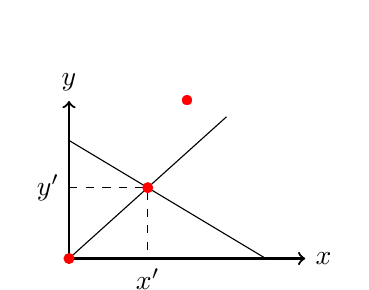
\begin{tikzpicture}
    \draw [<->,thick] (0,2) node (yaxis) [above] {$y$}
        |- (3,0) node (xaxis) [right] {$x$};
    \draw (0,0) coordinate (a_1) -- (2,1.8) coordinate (a_2);
    \draw (0,1.5) coordinate (b_1) -- (2.5,0) coordinate (b_2);
    \coordinate (c) at (intersection of a_1--a_2 and b_1--b_2);
    \draw[dashed] (yaxis |- c) node[left] {$y'$}
        -| (xaxis -| c) node[below] {$x'$};
    %
    \fill[red] (0,0) circle (2pt);
    \draw (0,0) node {\pdftooltip{\rule{0pt}{0.5cm}\rule{0.5cm}{0pt}}{Origin}};
    %
    \draw[red] (1.5,2) node {\pdftooltip{\textbullet}{1.5,2.0}};
    %
    \fill[red] (c) circle (2pt)
    let
        \p1 = (current path bounding box.south west),
        \p2 = (current path bounding box.north east)
    in
    node at (current path bounding box)
    {\pdftooltip{\rule{\dimexpr\x2-\x1\relax}{0pt}\rule{0pt}{\dimexpr\y2-\y1\relax}}%
    {This is the intersection point\textCR of the two lines!}};   
\end{tikzpicture}
\hspace{1cm}
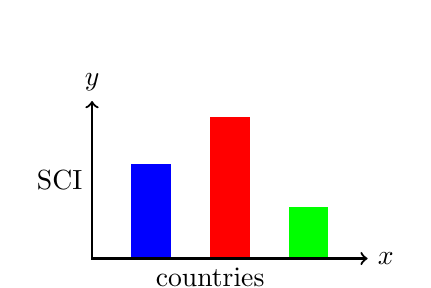
\begin{tikzpicture}
    \draw (1.5,0) node[below] {countries};
    \draw (0,1) node[left] {\pdftooltip{SCI}{Sausage Consumption Index}};
    \fill[blue] (0.5,0) rectangle (1,1.2)
    let
        \p1 = (current path bounding box.south west),
        \p2 = (current path bounding box.north east)
    in
    node at (current path bounding box)
    % these calculations are based on scale factor 1 otherwise use:
    % \dimexpr(scale factor)\dimexpr\x2-\x1\relax\relax
    {\pdftooltip{\rule{\dimexpr\x2-\x1\relax}{0pt}\rule{0pt}{\dimexpr\y2-\y1\relax}}%
    {USA: 120}};
    \fill[red] (1.5,0) rectangle (2,1.8)
    let
        \p1 = (current path bounding box.south west),
        \p2 = (current path bounding box.north east)
    in
    node at (current path bounding box)
    {\pdftooltip{\rule{\dimexpr\x2-\x1\relax}{0pt}\rule{0pt}{\dimexpr\y2-\y1\relax}}%
    {Germany: 180}};
    \fill[green] (2.5,0) rectangle (3,0.65)
    let
        \p1 = (current path bounding box.south west),
        \p2 = (current path bounding box.north east)
    in
    node at (current path bounding box)
    {\pdftooltip{\rule{\dimexpr\x2-\x1\relax}{0pt}\rule{0pt}{\dimexpr\y2-\y1\relax}}%
    {South Africa: 65}};
    \draw [<->,thick] (0,2) node (yaxis) [above] {$y$}
        |- (3.5,0) node (xaxis) [right] {$x$};
\end{tikzpicture}

\subsection{Misc. commands}

\subsubsection{\texorpdfstring{\cs{pdfcommentsetup}}{\textbackslash pdfcommentsetup}}
\label{sec:commentsetup}
With the command \cmd\pdfcommentsetup \margcs{\cmd\pdfcommentsetup\\\oarg{options}\marg{options}} you can reset the global options at any time. By using the optional option \styleoption{local} you can keep the reset local within a \LaTeX\ group.

\subsubsection{\texorpdfstring{\cs{listofpdfcomments}}{\textbackslash listofpdfcomments}}
\label{sec:listofpdfcomments}
The command \cmd\listofpdfcomments\margcs{\cmd\listofpdfcomments\oarg{options}} creates a list of the PDF comments to ease finding them. The command offers the following options:

\begin{itemize}
\item \styleoption{liststyle} specifies the list style. Possible option values are:
\begin{itemize}
\item \mco{AuthorSubject} (default)
\item \mco{AuthorSubjectDeadline}
\item \mco{SubjectAuthorComment}
\item \mco{SubjectAuthorCommentDeadline}
\item \mco{AuthorComment}
\item \mco{AuthorCommentDeadline}
\item \mco{SubjectComment}
\item \mco{SubjectCommentDeadline}
\item \mco{Comment}
\item \mco{CommentDeadline}
\end{itemize}


\item \styleoption{heading} specifies an alternative heading, e.\,g. \styleoption{heading}=\{List of comments\}.
\end{itemize}

\subsubsection{\texorpdfstring{\cs{setliststyle}}{\textbackslash setliststyle}}
\label{sec:setliststyle}
The command \cmd\setliststyle\margcs{\cmd\setliststyle\marg{name}} is necessary, if comments are used before \cmd\listofpdfcomments\ and you wish to have an alternative list style.

\subsubsection{\texorpdfstring{\cs{defineliststyle}}{\textbackslash defineliststyle}}
\label{sec:defineliststyle}
With the command \cmd\defineliststyle\margcs{\cmd\defineliststyle\\\marg{name}\marg{definition}} you can define new list styles, e.\,g.:

\medskip
\cmd\makeatletter\\
\cmd\defineliststyle\{MyListstyle\}\{\cmd\pc@lopt@subject\texttt{\textbackslash}\ \cmd\textcolor\{green\}\\\{(\cmd\pc@lopt@author)\}:\texttt{\textbackslash}\ \cmd\pc@lopt@comment\texttt{\textbackslash}\ \cmd\textcolor\{red\}\\\{(\cmd\pc@lopt@deadline)\}\\
\cmd\makeatother

\subsubsection{\texorpdfstring{\cs{defineavatar}}{\textbackslash defineavatar}}
\label{sec:defineavatar}
With the command \cmd\defineavatar \margcs{\cmd\defineavatar\marg{name}\marg{options}} you can create named predefined option lists, which can be later used in the comment commands with the option \styleoption{avatar}. With this option, it's easy for several authors of the same document to switch between different avatars, that is their graphical representation. 

\subsubsection{\texorpdfstring{\cs{definestyle}}{\textbackslash definestyle}}
\label{sec:definestyle}
With the command \cmd\definestyle \margcs{\cmd\definestyle\marg{name}\marg{options}} you can split up lists in personal and stylistic option lists (see \LinkEx). This option list can be loaded with the option \styleoption{style}.

\section{Printing comments and popups}
\label{sec:print}
Basically, \texttt{Adobe Reader} is able to print PDF annotations. Therefore, you have to choose 'Document and Markups' in the field 'Comments and Forms' of the print dialog. Additionally, you have to configure the menu 'Edit $\rightarrow$ Preferences... $\rightarrow$ Commenting $\rightarrow$ Print notes and pop-ups'. This entry exists since the release of \texttt{Adobe Reader X}. For older versions, the only possibility is to edit the configuration files itself. 

\begin{description}
\item[Windows:] the registry needs to be changed (on your own risk!)

Start the registry editor (\file{regedit.exe}) and open the following key, e.\,g. for \texttt{Adobe Reader 9.0}:

\texttt{HKEY\_CURRENT\_USER/Software/Adobe/Acrobat Reader/9.0/Annots/\newline cPrefs}

The key for other version will be similar, except version number and some letters in lower- or uppercase!

Open or create (with closed \texttt{Adobe Reader}) the key \newline\texttt{bprintCommentPopups} and change the value to 1 (dword).

\item[Linux:] open the configuration file:

\nolinkurl{~/.adobe/Acrobat/8.0/Preferences/reader_prefs}

with a text editor and change the entry 

{\texttt{/printCommentPopups\,[/b false]} to \texttt{/printCommentPopups\,[/b true]}}
\end{description}

Please note that only opened popups will be printed!

\end{document}
